\documentclass{article}
\usepackage{tikz, comment}
\usepackage{pifont}
\usepackage{fontspec, pgfplots}
\usetikzlibrary{arrows, decorations.markings, decorations.pathreplacing}
\begin{comment}
:Title: Not defined yet
:Tags: focus of a parabola;moment;directrix of a parabola;perimeter;apothem
:Prob: 0.5836;0.58;0.5647;0.5569;0.5534
:Author: Prof.Hu Ji-shan, HKUST
:Slug: No name yet

Description Here.........
\end{comment}
\begin{document}\centering 

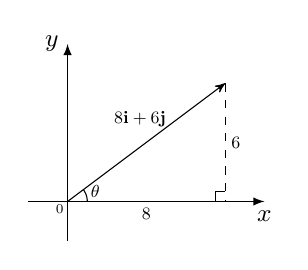
\begin{tikzpicture}[>=latex,xscale=.5*0.5, yscale=.5*0.5][font=\sf\small] 

%\draw[xstep=1cm,ystep=1cm,color=gray!80] (0, -1) grid (8, 8);

    	\foreach \x in {}
     		\draw (\x,2pt/2.5) -- (\x,-2pt/2.5)
			node[anchor=north] {\tiny$\x$}
			;

    	\foreach \x in {}
     		\draw (\x,2pt/1) -- (\x,-2pt/1)
			node[anchor=south] {\tiny$\x$}
			;
    	\foreach \y in {}
     		\draw (-2pt/1,\y) -- (2pt/1,\y)
			node[anchor=east] {\tiny $\y$}
			;

\draw[->] (-2, 0) -- (10, 0)node[below] {$x$} ;
\draw[->] (0, -2) -- (0, 8)node[left] {$y$} ;

\draw[->, >=stealth'] (0, 0) -- (8, 6)node[black, left, midway, pos=0.7, xshift=-2, yshift=0, scale=0.7]{$8{\bf i}+6{\bf j}$};

\draw[dashed] (8, 6)--(8, 0)node[black, right, midway, pos=0.5, xshift=0, yshift=0, scale=0.7]{$6$};

\node[below, scale=0.7] at (4, 0) {$8$};

\draw[black, samples=100, smooth, domain=0:36.9, variable=\t] 
		plot ({1*cos(\t)}, {1*sin(\t)}); 

\draw ({8-0.5}, 0)--++(0, 0.5)--++(0.5, 0); 


\node[xshift = 10, yshift = 3.5, scale=0.7] at (0, 0) {$\theta$};

\node[scale=0.7] at (-0.2/0.5, -0.2/0.5) {\scriptsize$0$};

\end{tikzpicture}
\end{document}